\section{Method}
\label{sec:method}

Figure~\ref{fig:overview} shows the stages of the pipeline on one discharge, and every stage runs with the same settings on every shot without any per-shot tuning.

\begin{figure}[t]
\centering
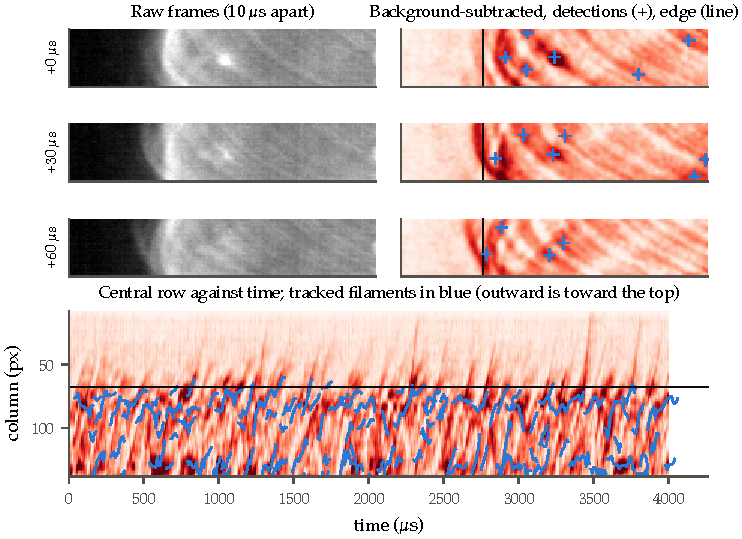
\includegraphics[width=\linewidth]{figs/fig_overview.pdf}
\caption{Pipeline stages on discharge 15235 (M6, 7~$\mu$s exposure), with three raw frames 30~$\mu$s apart and the corresponding background-subtracted frames with detections (crosses) and the edge column (line) in the top row, and the central row of the background-subtracted strip against time with tracked filaments overlaid in the bottom row, where filaments appear as inclined streaks that move toward the SOL (upward in this view).}
\label{fig:overview}
\end{figure}

\subsection{Strip geometry and the plasma edge}
A recording is an array of $n$ frames of $48 \times 256$ pixels with 10-bit depth, whose columns run across the plasma edge so that the SOL occupies one end of the strip and the core the other, with the end depending on how the camera was mounted in that campaign. The row-averaged brightness profile $p(t, x)$ is smoothed over 200 frames (2~ms) in time and $\sigma = 2$ columns in space, and the darker outer quarter of the columns is taken as the SOL side, which fixes a sign $s = \pm 1$ such that outward motion is $s\,\mathrm{d}x/\mathrm{d}t$. The edge column $x_{\rm half}(t)$ is the first column, scanning from the SOL side, at which $p$ exceeds the midpoint between the dark level, defined as the mean of the ten outermost SOL-side columns, and the interior level, defined as the median over the columns 40--75\% of the way across the strip from the SOL side, with linear sub-pixel interpolation. The limb peak $x_{\rm peak}(t)$ is the maximum of $p$ within 40 columns inboard of $x_{\rm half}$, refined by parabolic interpolation, and detections are referenced to $x_{\rm half}$ during processing and shifted to $x_{\rm peak}$ at aggregation, because the peak is the feature that the calibration in Section~\ref{sec:calibration} ties to the equilibrium.

\subsection{Background subtraction and detection}
Because filaments are transient, a per-pixel running minimum over 21 frames ($\pm 10$ frames, $\pm 100~\mu$s) estimates the quiescent background \citep{kirk2016filaments}, and the fluctuation image is the frame minus this background, passed through a $3 \times 3$ median filter and a Gaussian with $\sigma = 1$ pixel. The noise level $\sigma_n$ is $1.4826$ times the median absolute deviation of all fluctuation pixels in a block of 3{,}000 frames, pixels above $3\sigma_n$ are labelled into 8-connected components, and components smaller than 12 pixels are dropped. Each remaining component yields its intensity-weighted centroid $(x_c, y_c)$, its peak fluctuation, its orientation and major and minor axis lengths from its second central moments, and its radial width, which is measured on a chord as the number of columns at or above half the maximum of the fluctuation averaged over the five rows centred on $y_c$. The width is measured on a chord because filaments appear as inclined streaks and the column extent of a whole component grows with the tilt, and the signed SOL distance of a detection is $s\,(x_c - x_{\rm half})$.

\subsection{Tracking}
Detections in consecutive frames are linked by the Hungarian method \citep{kuhn1955hungarian}, with the Euclidean distance between centroids as the cost and a gate of 12 pixels per frame, which corresponds to about 4.5~cm or 4.5~km/s at the calibrated scale. Unmatched detections start new tracks, a track ends at the first frame without a match, and tracks with fewer than five detections (50~$\mu$s) are discarded. The radial velocity of a track in pixels per frame is the least-squares slope of $s\,x_c$ against frame index, with a standard error from the residuals, while its width is the median chord FWHM over the track and its SOL distance the median signed distance. Recordings are processed in blocks of 3{,}000 frames with a 60-frame overlap, and tracks that start in the overlap are dropped from the earlier block and recovered in the later one.

\subsection{Optical flow as an independent velocity}
As a check on the tracking, the velocity at each detection is also estimated by Lucas--Kanade optical flow \citep{lucas1981iterative}, in which Sobel spatial gradients and the frame difference in a $7 \times 7$ window around the centroid give a $2 \times 2$ least-squares system for the displacement between frames $f$ and $f + 1$, solved when its condition number is below $10^4$. The flow velocity of a track is the mean of the horizontal component over its detections with the sign $s$ applied, and because this estimate uses no assignment step and responds to the whole brightness profile around the centroid, agreement between the two estimates is evidence that neither is an artefact of its method.

\subsection{ELM detection}
Edge-localized modes (ELMs) eject large filaments that would dominate a velocity distribution, so they are detected from the midplane $D_\alpha$ monitor, sampled at 50--250~kHz depending on the campaign, as spikes where the residual after a 5~ms running median exceeds six times its robust standard deviation, with the time of each spike taken as the centre of mass of its samples. In some campaigns the monitor is coarsely digitized, with only tens of distinct values, which makes the robust standard deviation vanish, so the threshold is floored at six digitizer steps and at half the inter-ELM level. Because the $D_\alpha$ channel is absent or saturated in some discharges, the same detector is also applied to the frame-mean camera brightness, and a track that begins within 1~ms of a spike of either kind is flagged, while discharges with more than five $D_\alpha$ spikes inside the camera window are labelled ELMy. Flagged tracks are excluded from all statistics, and the parameter dependences in Section~\ref{sec:analysis} use the non-ELMy discharges only.

\subsection{Pixel scale from the equilibrium}
\label{sec:calibration}
The archive gives no spatial calibration for the strip recordings, and the scale is therefore recovered from the data. Because the limb peak sits where the line of sight is tangent to the flux surfaces at the LCFS, its sensor column should move with the outboard LCFS radius $R_{\rm LCFS}$ from EFIT, and the slope of column on radius is the inverse pixel scale. Within a single discharge $R_{\rm LCFS}$ moves by only a few centimetres during the flat top, the EFIT reconstruction is least reliable during ramp-up and termination, and the brightness profile changes shape as the density rises, so a within-shot regression is unstable (Appendix~\ref{app:calibration}). Between discharges, by contrast, the plasma position varies by 10--20~cm while the camera and its optics stay fixed through a campaign, which gives a much longer lever arm.

For each discharge, $R_{\rm LCFS}$ is taken at every EFIT time inside the flat top as the largest major radius of the EFIT boundary contour within 5~cm of the magnetic-axis height, $x_{\rm peak}$ is taken from the profile smoothed over 2~ms, and EFIT samples whose $R_{\rm LCFS}$ differs by more than 8~cm from the flat-top median are dropped as unconverged. Each discharge then contributes one point, its median $x_{\rm peak}$, converted to sensor coordinates by adding the region-of-interest offset recorded in the camera metadata, against its median $R_{\rm LCFS}$. A camera configuration is defined as the combination of campaign, view string in the camera metadata, and region-of-interest offset, because a change in any of these can mean a change of lens, pointing, or sensor region. A configuration with at least 8 discharges and at least 3~cm of spread in $R_{\rm LCFS}$ receives its own Theil--Sen slope \citep{sen1968estimates}, which is kept if its sign agrees with $s$, the Spearman correlation satisfies $|\rho| \ge 0.5$, and the bootstrap interval excludes zero. Every other configuration uses the pooled slope of its campaign, fitted on all configurations of the campaign after the mean $R_{\rm LCFS}$ and mean column of each configuration are subtracted to remove the per-configuration intercepts, and in all cases the 95\% intervals come from 2{,}000 bootstrap resamples of discharges within configurations \citep{efron1993bootstrap} and the scale is the inverse of the slope magnitude.

\subsection{Physical units and track selection}
The radial velocity of a track is $v_r = s\,\dot x_c \times f_{\rm frame} \times \ell$, where $\ell$ is the pixel scale, and its radial width is $\delta_r = \mathrm{FWHM} \times \ell$, while the SOL distance is measured from $x_{\rm peak}$ using the per-shot median offset $x_{\rm peak} - x_{\rm half}$. A track enters the statistics if its median position lies between 10 pixels inboard and 40 pixels outboard of the limb peak (3--5~cm inboard to 11--21~cm outboard, depending on the scale of the configuration), its velocity standard error is below 0.5 pixels per frame, its width is finite, it begins inside the plasma flat top, and it is free of an ELM flag. A discharge enters the shot-level statistics if it has at least 50 such tracks with $v_r > 0$, which keeps the per-discharge medians stable.

\subsection{Statistics}
All central values are medians with 95\% bootstrap intervals from 2{,}000 resamples, and slopes are Theil--Sen estimates in $\log_{10}$--$\log_{10}$ coordinates with the 95\% interval of the estimator, reported together with Spearman's $\rho$. The velocity--size slope is computed per discharge and also pooled, and for the pooled fit the $v_r$ and $\delta_r$ of each track are divided by the medians of its discharge so that differences between discharges in the pixel scale or the plasma conditions do not create a spurious correlation. The correction for exposure blur replaces $\delta_r$ by $\delta_{\rm corr} = (\delta_r^2 - (v_r t_{\rm exp})^2)^{1/2}$, which treats the smear as a Gaussian of width $v_r t_{\rm exp}$ added in quadrature, before the slope is refitted. Parameter dependences are Theil--Sen slopes of the per-discharge median $v_r$ and $\delta_r$ on plasma current, Greenwald fraction, and injected beam power, with the beam power offset by 0.05~MW so that Ohmic discharges enter the log fit.

The two-region normalization requires $T_e$ and $n_e$ at the LCFS, $B$, $q_{95}$, and $R$, and the temperature comes from the Thomson scattering profile, from the edge system where it exists and the core system otherwise, interpolated at $R_{\rm LCFS}$ and taken as the median over the flat top, with $T_e = \teDefault$~eV assumed and marked as such when no profile reaches the LCFS. The separatrix density $n_{e,\rm sep}$ is taken as half the line-averaged density, $B$ as the vacuum toroidal field at the magnetic axis scaled by $R_{\rm axis}/R_{\rm LCFS}$, and the connection length as $L_\parallel = \pi q_{95} R_{\rm axis}$, while the filament radius in the model is half the measured FWHM, $a = \delta_r/2$, and $\nu_{ei}$ follows the NRL formulary \citep{nrl2019formulary} with deuterium ions.
